
\documentclass[letterpaper,11pt]{article}

\usepackage{amsmath}
\usepackage{amssymb}
\usepackage[margin=1in,nohead]{geometry}
\usepackage{tikz}

\newcommand{\sR}{\mathbb{R}}

\newcommand{\figlab}[1]{\label{fig:#1}}
\newcommand{\figref}[1]{Figure~\ref{fig:#1}}

\tikzstyle{coordaxis}=[draw=red!50!black, thick, ->]
\tikzstyle{mapping}=[draw=blue!50!black, thick, ->]
\tikzstyle{connect}=[draw=green!50!black, thick, ->]

\author{Carsten Burstedde}
\title{Documentation on octree and quadrant connectivity}

\begin{document}

\maketitle

\section{Mappings between octrees and physical space}

See \figref{octreemap} for an illustration.

\begin{figure}[b!]
\centering
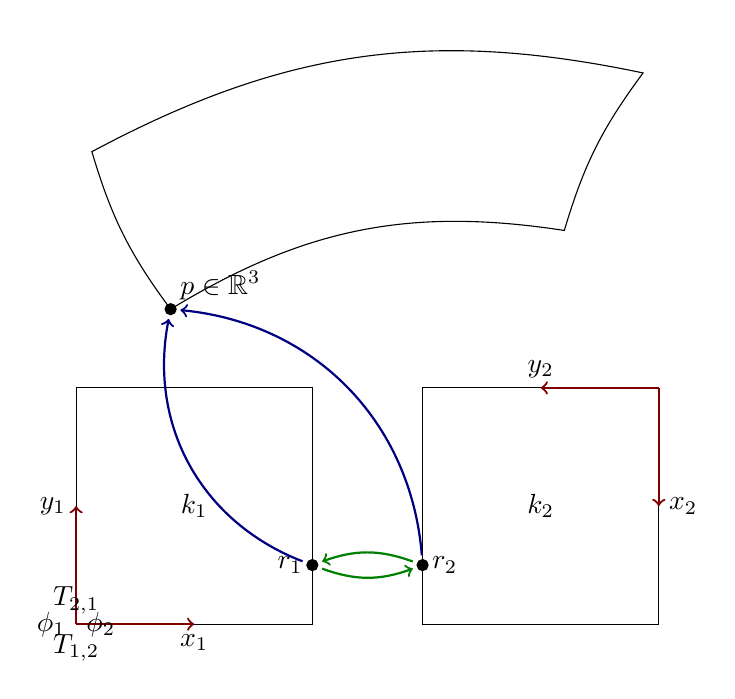
\begin{tikzpicture}
  % first tree
  \begin{scope}[xshift=0cm]
  \draw (0,0) rectangle (3,3) node (m1) [midway] {$k_1$};
  \draw [style=coordaxis] (0,0) -- (1.5,0) node [below] {$x_1$};
  \draw [style=coordaxis] (0,0) -- (0,1.5) node [left] {$y_1$};
  \filldraw (3,0.75) node (r1) {} circle (2pt) node [left] {$r_1$};
  \end{scope}

  % second tree
  \begin{scope}[xshift=4.4cm]
  \draw (0,0) rectangle (3,3) node (m2) [midway] {$k_2$};
  \draw [style=coordaxis] (3,3) -- (3,1.5) node [right] {$x_2$};
  \draw [style=coordaxis] (3,3) -- (1.5,3) node [above] {$y_2$};
  \filldraw (0,0.75) node (r2) {} circle (2pt) node [right] {$r_2$};
  \end{scope}

  % physical space
  \begin{scope}[xshift=1.2cm, yshift=4cm]
  \draw (0,0) to [bend left=20] (5,1) node (pm1) [midway] {}
              to [bend left=10] (6,3)
              to [bend right=20] (-1,2) node (pm2) [midway] {}
              to [bend right=10] (0,0);
  \draw (pm1.center) to [bend left=5] (pm2.center) node (pmm) [pos=.25] {};
  \filldraw (pmm) circle (2pt) node [above right] {$p \in \sR^3$};
  \end{scope}

  % connections
  \draw [connect] (r1) to [bend right=20] (r2)
        node [midway, below] {$T_{1,2}$};
  \draw [connect] (r2) to [bend right=20] (r1)
        node [midway, above] {$T_{2,1}$};
  \draw [mapping] (r1) to [bend left=40] (pmm) node [pos=0.55, left] {$\phi_1$};
  \draw [mapping] (r2) to [bend right=40] (pmm) node [pos=0.6, right] {$\phi_2$};

\end{tikzpicture}
\caption{%
Two octrees $k_1$ and $k_2$ and their individual octree coordinate systems
(red).  Quadrant coordinates at subdivision level $\ell \ge 0$ (not shown) are
discrete numbers that are integer multiples of $2^{-\ell}$.  In this example
the octrees connect through a common face, which defines coordinate
transformations $T_{1,2} = T_{2,1}^{-1}$ across this face.  The octree points
$r_1 = (1, \frac14)$ and $r_2 = (\frac34, 1)$ are identified: $T_{i,j}(r_i) =
r_j$ (green).  This identification is specified solely based on the
connectivity relation between the two octrees.  The functions $T_i$ can be
implemented in integer arithmetic, entirely without using physical coordinates.
To map the octrees to physical space, geometry transformations $\phi_1$,
$\phi_2$ (blue) are introduced that satisfy the compatibility condition $p =
\phi_1 (r_1) = \phi_2 (r_2)$.  This offers the alternate identification
criterion $r_j = (\phi_j ^{-1} \circ \phi_i) (r_i)$.  However, this approach is
not recommended since it is much more expensive and, more importantly, depends
on the floating-point functions $\phi_i$ that suffer from roundoff error and
make it difficult to determine uniqueness.
}
\figlab{octreemap}
\end{figure}

\end{document}
